\chapter{배포 전·후의 학습 regime 지도}
\label{bg:chapter-training-regimes}

\section{Regime를 네 질문으로 구분한다}

학습 이름이 많아 보이지만 네 질문으로 정리할 수 있다. (1) 언제 학습하는가, (2) 어떤
데이터를 쓰는가, (3) 어떤 상태가 바뀌는가, (4) 무엇이 serving artifact가 되는가. 이 네
항목이 같다면 이름이 달라도 시스템 workload는 비슷하고, 하나라도 다르면 compute와
governance가 달라진다.

\begin{figure}[htbp]
  \centering
  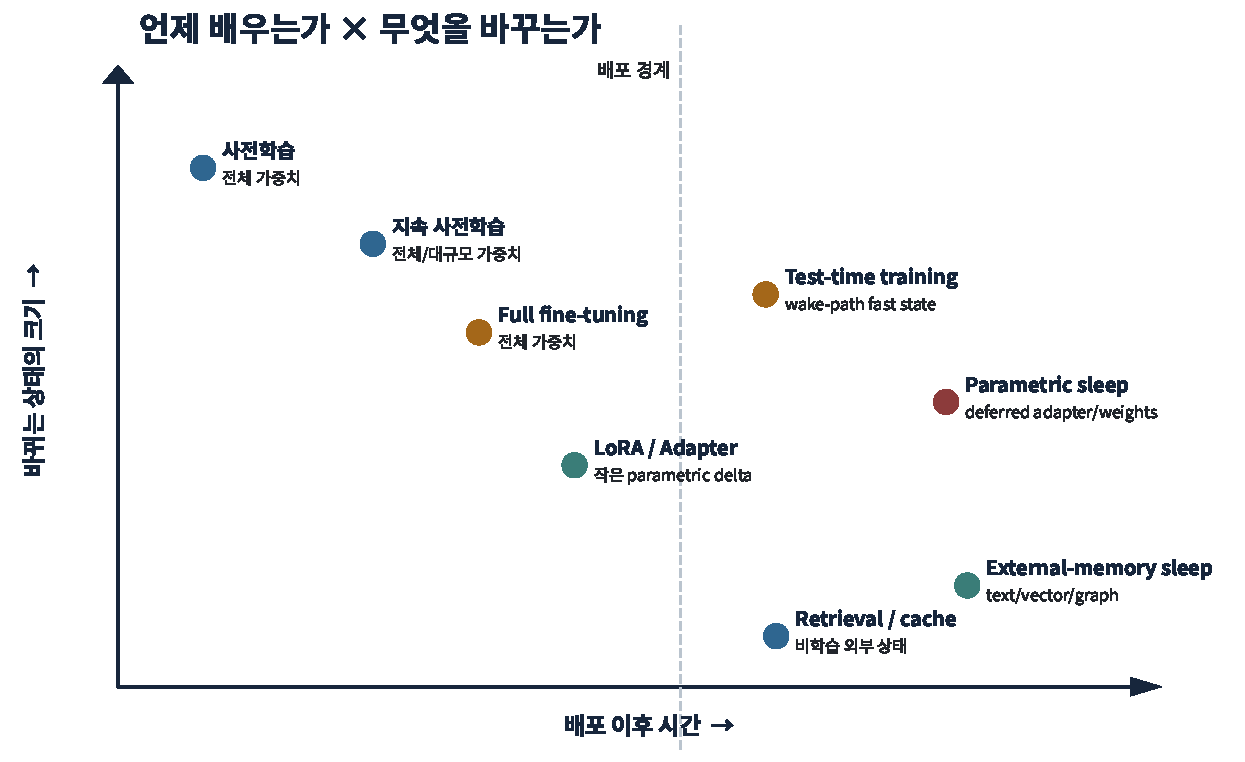
\includegraphics[width=0.95\textwidth]{figures/training-regimes.pdf}
  \caption{배포 시점과 변경 상태 크기로 본 training regime. Test-time training은 wake-path,
  sleep-time training은 deferred path에 놓이지만 둘 다 외부 기억과 parametric 상태를 선택할 수 있다.}
  \figsource{Original synthesis; SRC-STC-0014, SRC-STC-0021, SRC-STC-0030}{가로축은 배포 이후 시간, 세로축은 변경 상태 크기이고 사전학습, fine-tuning, LoRA, TTT, parametric sleep, external-memory sleep이 표시된다.}
  \label{fig:bg-training-regimes}
\end{figure}

\section{Pre-training과 continued pre-training}

\concept{pretraining}{사전학습}은 대규모 corpus에서 범용 representation과 생성 능력을
형성한다. language model은 보통 다음 token의 negative log-likelihood를 줄인다.

\begin{equation}
  \mathcal L_{\mathrm{LM}}(\theta)
  =-\sum_{t=1}^{T}\log p_\theta(x_t\mid x_{<t}).
  \label{eq:bg-lm-loss}
\end{equation}

한 번의 pre-training은 data curation, tokenizer, distributed optimizer, checkpoint,
evaluation이 결합된 장기 run이다. 모든 weight와 optimizer state가 sharding되고, 장애 시
재시작 가능한 checkpoint chain이 필요하다.

\concept{continued-pretraining}{지속 사전학습}은 이미 훈련된 model을 새 domain corpus나
최신 corpus로 계속 학습한다. 일반적으로 pre-training과 같은 self-supervised objective를
쓰지만 learning rate, data mixture, replay 비율을 조정한다. domain 지식은 늘 수 있으나
기존 능력과 언어 분포를 손상할 수 있어 base corpus replay와 broad evaluation이 필요하다.
Global knowledge refresh에는 유력하지만 per-user memory를 매 interaction마다 넣기에는
batching·privacy·rollback 단위가 너무 거칠 수 있다.

\section{Full fine-tuning과 instruction tuning}

\concept{fine-tuning}{미세조정}은 pretrained model을 더 좁은 데이터나 행동 목표에 맞게
추가 학습한다. full fine-tuning은 대부분 또는 모든 weight를 trainable하게 둔다. 작은
dataset에서도 높은 표현력을 갖지만, gradient·optimizer state·checkpoint가 full model
scale이고, 여러 사용자 variant를 독립 보관하기 어렵다.

\concept{instruction-tuning}{지시 튜닝}은 instruction--response pair로 원하는 task format과
behavior를 학습한다. 정답 token에 대한 supervised loss가 대표적이다. 답변 style과 tool
protocol을 형성하기 좋지만, interaction log를 그대로 정답으로 간주하면 사용자 오류와
assistant hallucination을 재학습할 수 있다. Sleep dataset은 raw transcript가 아니라
verifier를 통과한 target과 negative example을 포함해야 한다.

\section{Preference optimization}

\concept{preference-optimization}{선호 최적화}는 두 출력 중 어느 것이 더 나은지에 대한
preference를 사용한다. reward model을 따로 학습하고 policy를 RL로 최적화할 수도 있고,
chosen/rejected pair에서 직접 loss를 만들 수도 있다. 중요한 것은 algorithm 이름보다
reference behavior, preference provenance, distribution shift다.

개인화 sleep에서는 ``사용자가 한번 수정했다''는 사건을 영구 선호로 확대하면 위험하다.
상황적 요청, 장기 선호, 조직 policy를 구분해야 한다. preference update는 probability를
바꾸기 때문에 사실 memory와 달리 정확한 source sentence 하나로 rollback하기 어렵다.

\begin{table}[htbp]
\centering
\caption{대표 training regime의 상태와 비용}
\label{tab:bg-training-regimes}
\small
\begin{tabularx}{\textwidth}{L{0.16\textwidth}L{0.17\textwidth}L{0.18\textwidth}YY}
\toprule
Regime & 주 데이터 & Trainable state & Serving artifact & 주요 실패 \\
\midrule
pre-training & web/code/multimodal corpus & 전체 weights + optimizer & base checkpoint & bias, contamination, huge cost \\
continued PT & domain/latest corpus + replay & 전체 또는 대규모 weights & refreshed checkpoint & domain drift, forgetting \\
full FT & labeled task/user data & 전체 weights & full variant & interference, storage explosion \\
instruction tuning & instruction-response & 전체 또는 PEFT & aligned checkpoint/adapter & imitation of bad targets \\
preference opt. & comparisons/reward & policy + optional reward model & aligned policy & reward hacking, preference drift \\
LoRA/adapter & task/user examples & 작은 delta/module & base + delta & adapter conflict, base churn \\
TTT & current input/stream & fast weights/state & session state & latency, instability \\
sleep training & accumulated episodes & chosen destination state & validated next version & stale data, rollback, fleet cost \\
\bottomrule
\end{tabularx}
\end{table}

\section{Sleep-time은 새로운 objective가 아니라 lifecycle 축이다}

Sleep-time compute는 특정 optimizer나 architecture의 이름이 아니다. 같은 LoRA update도
response를 만들기 전에 current query로 수행하면 test-time training이고, response 이후
여러 episode를 정리해 다음 session의 adapter를 만들면 sleep-time training이다. 반대로
background process가 text summary와 graph edge만 갱신한다면 training kernel 없이도 sleep
lifecycle에 속한다.

따라서 infra를 분류할 때 ``training cluster인가 inference cluster인가''만 묻지 않는다.
wake critical path, deferred transformation path, persistent state destination, validation and
publication plane을 따로 본다. 이 구분이 있어야 sleep job을 spare GPU에 단순 배치하는 접근과
state-aware lifecycle system을 구별할 수 있다.
